\documentclass[a4paper, 12pt]{article}
\usepackage[hagavi]{azzam}

\begin{document}
\title{Kompilasi Geometri Untuk OSN SMP V10.08}
\maketitle
\begin{enumerate}
\section{Geometri Tiga Dimensi}
    \item (OSP SMP 2016) Diberikan Kubus $ABCD.EFGH$ dengan panjang rusuk $2~cm$. Titik $P$ terletak pada perpanjangan $HE$ sehingga $PE = 1~cm$. Tentukan jarak titik $P$ ke bidang yang memuat segitiga $AHF$.
    \begin{center}
        \begin{tikzpicture}
        \coordinate (D_cube) at (1,1.5); % Front-bottom-left
        \coordinate (C_cube) at (4,1.5); % Front-bottom-right
        \coordinate (B_cube) at (3,0);    % Back-bottom-right
        \coordinate (A_cube) at (0,0);    % Back-bottom-left
    
        \coordinate (H_cube) at (1,4.5); % Front-top-left
        \coordinate (G_cube) at (4,4.5); % Front-top-right
        \coordinate (F_cube) at (3,3);    % Back-top-right
        \coordinate (E_cube) at (0,3);    % Back-top-left
    
        % Draw dashed lines
        \draw[dashed] (D_cube) -- (A_cube); % Back to front bottom-left
        \draw[dashed] (D_cube) -- (C_cube); % Back bottom-left to back bottom-right
        \draw[dashed] (D_cube) -- (H_cube); % Back bottom-left to back top-left
    
        % Draw solid lines
        \draw (A_cube) -- (B_cube) -- (C_cube); % Front bottom and bottom-right
        \draw (A_cube) -- (E_cube) -- (F_cube) -- (B_cube); % Front face
        \draw (G_cube) -- (C_cube); % Right face
        \draw (E_cube) -- (H_cube) -- (G_cube) -- (F_cube); % Top face
        \draw (E_cube) -- (H_cube); % Left top edge (already part of top face)
    
        % Draw the additional line segments (diagonals/internal)
        \draw (A_cube) -- (H_cube);
        \draw (H_cube) -- (F_cube);
        \draw (A_cube) -- (F_cube); 
    
        % Draw line segment P-E
        % Extend E-A to P
        \coordinate (P_point) at ($ (E_cube)!-0.5!(H_cube) $);
        \draw (P_point) -- (E_cube);
        
        % Label the points
        \node[above right] at (D_cube) {D};
        \node[below left] at (A_cube) {A};
        \node[below right] at (B_cube) {B};
        \node[below right] at (C_cube) {C};
        
        \node[above left] at (E_cube) {E};
        \node[above right] at (F_cube) {F};
        \node[above right] at (G_cube) {G};
        \node[above left] at (H_cube) {H};
        
        \node[left] at (P_point) {P};
    
    \end{tikzpicture}
    \end{center}

    \item (OSN SMP 2022) Kubus $ABCD.EFGH$ memiliki volume 1 liter. Titik $I$ pada $BF$ dan titik $J$ pada $CG$ sehingga $IJ \parallel BC$. Titik $K$ dan $L$ adalah titik Tengah $EH$ dan $FG$ berturut-turut. Titik $O$ pada bidang $IJK$ yang paling dekat ke $L$. jarak $F$ ke garis $IK$ adalah $\frac{5}{2}\sqrt{70}$. Tentukan volume limas $L.OIJ$.

    \item (OSN SMP 2024) Panjang salah satu rusuk dari suatu balok adalah $7 + \sqrt{3}~cm$ dan luas permukaannya $176 cm^2$. Volume balok adalah $V~cm^3$ dan total panjang rusuk adalah $k~cm$, dengan $V$ dan $k$ merupakan bilangan bulat. Tentukan panjang diagonal ruang balok tersebut.

    \item (OSN SMP 2016) Diberikan kubus $ABCD.EFGH$ dengan panjang rusuk 1 dm. Terdapat persegi $PQRS$ pada bidang diagonal $ABGH$ dengan titik $P$ pada $HG$ dan $Q$ pada $AH$ seperti ditunjukkan pada gambar di bawah. Titik $T$ adalah titik pusat persegi $PQRS$. Garis $HT$ diperpanjang sehingga memotong garis diagonal $BG$ di $N$. Titik $M$ adalah proyeksi $N$ terhadapat $BC$. Tentukan volume prisma terpancung $DCM.HGN$.
    \begin{center}
    \begin{tikzpicture}[scale=3.5]
        % Define the coordinates for the cube vertices
        \coordinate (D) at (0.5,0.5);
        \coordinate (A) at (0, 0);
        \coordinate (C) at (1.5, 0.5);
        \coordinate (B) at ($(A)+(C)-(D)$);
        \coordinate (H) at (0.5, 1.5);
        \coordinate (E) at ($(A)+(H)-(D)$);
        \coordinate (G) at ($(C)+(H)-(D)$);
        \coordinate (F) at ($(B)+(H)-(D)$);

        % Find intersection point N
        \coordinate (N) at ($(G)!0.5!(B)$);
        % Define center T
        \coordinate (T) at ($(H)!0.3!(N)$);

        % Define points P, Q, R, S based on visual placement
        \coordinate (P) at ($(H)!0.3!(G)$);
        \coordinate (Q) at ($(H)!0.15!(A)$); % Q is on AH
        \coordinate (R) at ($(T)!-1.0!(P)$);
        \coordinate (S) at ($(T)!-1.0!(Q)$); % S is on GB
        
        % Draw the square PQRS (some edges dotted)
        \draw[thick] (Q) -- (P) -- (S);
        \draw[thick] (Q) -- (R) -- (S);

        % Define line paths for intersection
        \path[name path=HT_line] (H) -- ($(H)!1.5!(T)$);
        \path[name path=BG_line] (B) -- (G);

        % Find projection M on BC
        % For a standard cube, projection of N(nx,ny,nz) onto line BC is (nx, s, 0)
        % In our perspective, we find the point on BC that has the same 'depth' as N.
        \coordinate (M) at ($(B)!0.5!(C)$); % Project N onto the line BC

        % Draw additional lines
        \draw[thick] (P) -- (R);
        \draw[thick] (S) -- (Q);
        \draw[thick, dotted] (H) -- (N); % The full line HTN
        
        % Draw the prism shape DCM.HGN
        \draw[thick] (N) -- (M);
        \draw[thick] (C) -- (M);
        \draw[thick] (D) -- (C); % Already drawn
        \draw[thick] (H) -- (G); % Already drawn
        \draw[thick] (G) -- (N);
        \draw[thick, dotted] (H) -- (D); % Dotted
        \draw[thick] (G) -- (C); % Already drawn

        
        \draw[thick, dotted] (D) -- (M);
        \draw[thick, dotted] (H) -- (A);
        
        \draw[thick] (D) -- (A);
        \draw[thick] (D) -- (C);
        \draw[thick] (D) -- (H);
        \draw[thick] (E) -- (A);

    
        \draw[thick] (E) -- (F) -- (G) -- (H) -- cycle;
        \draw[thick] (A) -- (B) -- (C);
        \draw[thick] (B) -- (F);
        \draw[thick] (C) -- (G);
        \draw[thick] (E) -- (H);
        \draw[thick] (G) -- (B);

        % Label all the points
        \foreach \point/\pos in {A/left, B/below, C/right, D/below, E/left, F/above, G/right, H/left, P/above, Q/left, R/below, S/right, T/above, M/right, N/right}
        {
            \node[\pos] at (\point) {$\point$};
        }
    \end{tikzpicture}
    \end{center}

    \item (OSN SMP 2023) Terdapat sebuah kubus $ABCD.EFGH$ yang diletakkan dengan sisi $ABCD$ berada di lantai. Kubus itu diangkat sehingga posisi titik A tetap dan diagonal bidang ABGH tegak lurus lantai. Jarak titik $B$ dan titik $H$ ke lantai adalah 4 dan 12 berturut-turut. Kubus itu dipotong menjadi tiga bagian oleh dua bidang sejajar lantai dengan bidang pertama melalui $B$ dan bidang kedua berjarak 14 ke lantai. Tentukan volume terbesar dari ketiga bagian tersebut.

    \item (OSN SMP 2016) Diberikan kubus ABCD.EFGH dengan panjang rusuk 1 dm. Terdapat persegi PQRS pada bidang diagonal ABGH dengan titik P pada HG dan Q pada AH seperti ditunjukkan pada gambar di bawah. Titik T adalah titik pusat persegi PQRS. Garis HT diperpanjang sehingga memotong garis diagonal BG di N. Titik M adalah proyeksi N terhadapat BC. Tentukan volume prisma terpancung DCM.HGN.
    
\section{Angle Chasing}
    \item Jika $I$ adalah titik pusat lingkaran dalam atau titik bagi (incenter) dari $\triangle ABC$ maka buktikan bahwa
        $\angle BIC = 90^\circ + \frac{1}{2}A.$

    \item Misalkan $ABCDE$ adalah sebuah segilima konveks sedemikian sehingga $BCDE$ adalah persegi dengan pusat $O$ dan $\angle A = 90^\circ$. Buktikan bahwa $\overline{AO}$ membagi dua sama besar $\angle BAE$.

    \item Misalkan $O$ dan $H$ masing-masing menyatakan titik pusat lingkaran luar dan titik tinggi dari sebuah segitiga lancip $\triangle ABC$. Tunjukkan bahwa $\angle BAH = \angle CAO$.

    \item (OSN SMP 2003) Perhatikan gambar susunan tiga persegi di bawah. 
    
    Buktikan bahwa $\angle BAX+\angle CAX=45^{\circ}$.
    
        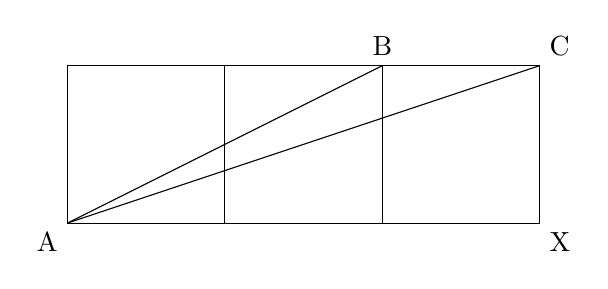
\begin{tikzpicture}[scale=1]
        % Define the unit width of each square
        \def\unitw{2} 
        
        % Draw the main rectangle (3 squares wide, 1 square high)
        \draw (0,0) rectangle (3*\unitw, \unitw);
        
        % Draw vertical lines for the squares
        \draw (\unitw,0) -- (\unitw,\unitw);
        \draw (2*\unitw,0) -- (2*\unitw,\unitw);
        
        % Draw the diagonal lines from A
        \draw (0,0) -- (2*\unitw, \unitw); % Line to B's position
        \draw (0,0) -- (3*\unitw, \unitw); % Line to C's position
        
        % Place the labels
        \node[below left] at (0,0) {A};
        \node[above] at (2*\unitw, \unitw) {B};
        \node[above right] at (3*\unitw, \unitw) {C};
        \node[below right] at (3*\unitw, 0) {X};
    \end{tikzpicture}

    \item (OSN SMP 2020) Misalkan AB sebagai diameter lingkaran dan P titik diluar lingkaran. Garis PQ dan PR menyinggung lingkaran di titik Q dan R. Garis PH berpotongan tegak lurus dengan garis AB di H dan PH berpotongan AR di S. Jika $\angle QPH=40^{\circ}$ dan $\angle QSA=30^{\circ}$ tentukan $\angle RPS$.
        
\section{Length Chasing}
    \item (Teorema Pitot) Misalkan $ABCD$ adalah sebuah segiempat. Jika sebuah lingkaran dapat menyinggung keempat sisinya, buktikan bahwa $AB + CD = BC + DA$.
    \begin{figure}[H]
        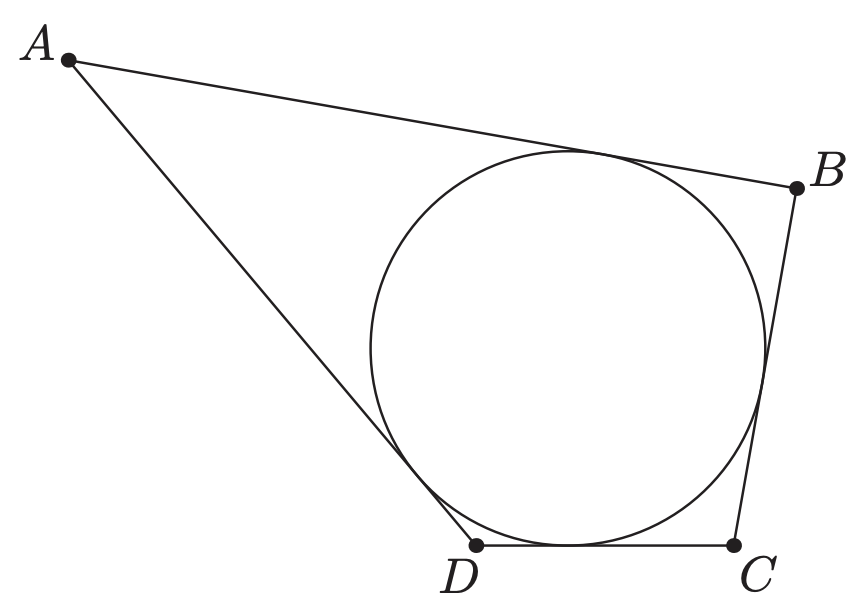
\includegraphics[width=0.4\linewidth]{0Figure/pitot-theorem.png}
    \end{figure}

    \item (OSN SMA 2002)
    Diberikan segitiga $ABC$ dengan $AC > BC$. Pada lingkaran luar segitiga $ABC$ terletak titik $D$ yang merupakan titik tengah busur $AB$ yang memuat titik $C$. Misalkan $E$ adalah titik pada $AC$ sehingga $DE$ tegak lurus pada $AC$. Buktikan bahwa $AE = EC + CB$.

    \item (OSN SMP 2022) Diketahui ABCD jajargenjang. Sebuah lingkaran dengan pusatnya pada perpotongan diagonal AC dan BD menyinggung AB dan CD. Lingkaran tersebut digeser sehingga menyentuh BC. Lingkaran hasil memotong diagonal BD di titik P dan Q. Jika $BP=9$, $PQ=27$, dan $DQ=48$. Tentukan luas daerah jajargenjang yang belum pernah disentuh lingkaran.

\section{Luas}
    \item (OSN SMP 2009) Pada suatu segitiga ABC, titik D terletak pada sisi AB dan titik E terletak pada sisi AC. Tunjukkan bahwa $\frac{\text{Luas } \triangle ADE}{\text{Luas } \triangle ABC} = \frac{AD \times AE}{AB \times AC}$.

    \item (OSN SMP 2021) Diketahui daerah segi empat ABCD dengan $AB=2$ cm, $BC=8$ cm, $CD=6$ cm, $DA=7$ cm, terbagi menjadi dua daerah segitiga oleh $\overline{AC}$ yang panjangnya 9 cm. lingkaran dalam kedua segitiga menyinggung $\overline{AC}$ di titik E dan F. Jika titik pusat masing-masing lingkaran dalam segitiga adalah M dan N, serta luas daerah segitiga EFM adalah $L \text{ cm}^{2}$, tentukan nilai maksimum dari $L^{2}$.



    \item (OSN SMP 2024) Perhatikan gambar segitiga ABC berikut.
    \begin{figure}[H]
    \centering
    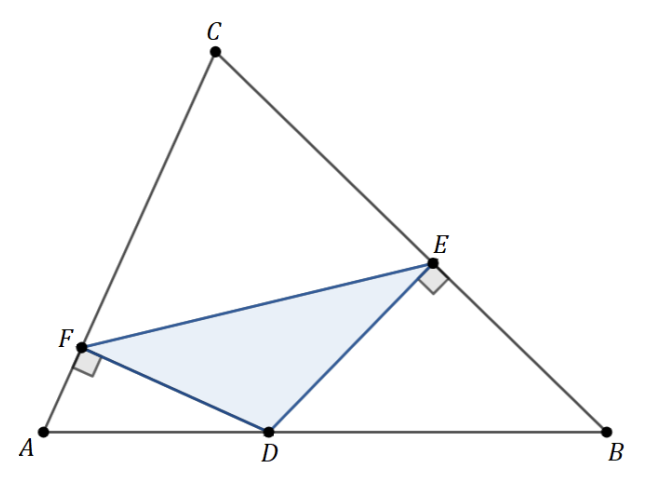
\includegraphics[scale=0.5]{0Figure/osn-smp-2024-3.png}
    \end{figure}
    Panjang sisi $BC=12$ cm dan $AC=8$ cm. Titik D, E, dan F berada pada sisi AB, BC, dan AC. Jika $DE=4$ cm, $AD:AB=1:3$, serta $\angle DEB$ dan $\angle DFA$ adalah sudut siku-siku, tentukan luas daerah segitiga DEF.

    \item (OSN SMP 2023) Diberikan sebuah segienam ABCDEF dengan panjang sisi 8 cm. pada setiap sisi, dibuat setengah lingkaran seperti pada gambar. Tentukan total luas daerah yang diarsir?
    \begin{figure}[H]
    \centering
    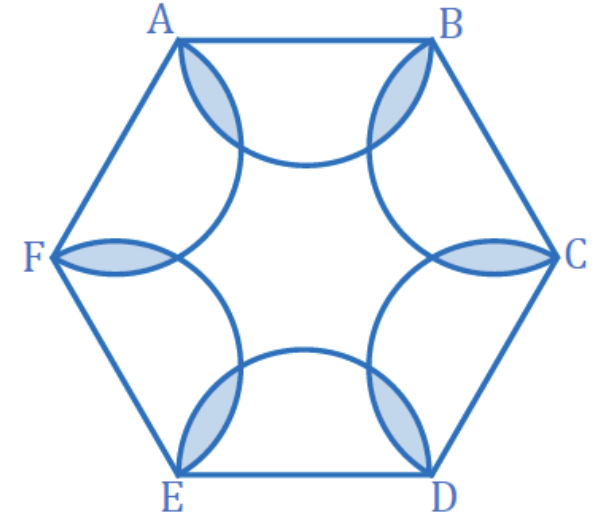
\includegraphics[scale=0.5]{0Figure/osn-smp-2023-1.png}
    \end{figure}

    \item (OSN SMA 2009) Pada segitiga $ABC$, titik-titik $D, E$ dan $F$ berturut-turut terletak pada segmen $BC, CA,$ dan $AB$. Nyatakan $P$ sebagai titik perpotongan $AD$ dan $EF$. Tunjukkan bahwa
    $$
    \frac{AB}{AF} \times CD + \frac{AC}{AE} \times BD = \frac{AD}{AP} \times BC
    $$
    
    \item (OSN SMA 2006)
    Pada segitiga $ABC$, $M$ adalah titik tengah $BC$ dan $G$ adalah titik berat segitiga $ABC$. Sebuah garis $l$ melalui $G$ memotong ruas garis $AB$ di $P$ dan ruas garis $AC$ di $Q$, dimana $P \neq B$ dan $Q \neq C$. Jika $[XYZ]$ menyatakan luas segitiga $XYZ$, tunjukkan bahwa
    $$
    \frac{[BGM]}{[PAG]} + \frac{[CMG]}{[QGA]} = \frac{3}{2}
    $$

    
    \section{Campur}


    \item (OSN SMP 2017) Terdapat 5 titik yang berbeda, $T_{1}$, $T_{2}$, $T_{3}$, $T_{4}$ dan $T$ pada sebuah lingkaran L. Misalkan $t_{ij}$ adalah jarak titik $T$ ke garis $T_{i}T_{j}$ atau perpanjangannya. Buktikan bahwa $\dfrac{t_{ij}}{t_{jk}}=\dfrac{TT_{i}}{TT_{k}}$ dan $\dfrac{t_{12}}{t_{24}}=\dfrac{t_{13}}{t_{34}}$.
    \newline
    \begin{tikzpicture}[scale=2]
        % Define the center and radius of the circle
        \coordinate (O) at (0,0);
        \def\R{1.5}
    
        % Define the points on the circle for the polygon
        % (Angles chosen to roughly match the input image)
        \coordinate (T1) at (180:\R);
        \coordinate (T2) at (220:\R);
        \coordinate (T3) at (320:\R);
        \coordinate (T4) at (30:\R);
        \coordinate (T)  at (100:\R); % The top point T
    
        % Draw the circle
        \draw (O) circle (\R);
    
        % Draw the polygon segments
        \draw (T1) -- (T2) -- (T3) -- (T4) -- (T) -- cycle; % This forms a pentagon
    
        % Draw the perpendicular from T1 to the tangent
        \tkzDefPointBy[projection = onto T1--T2](T)
        \tkzGetPoint{P_T1_tangent}
        \draw[dashed] (T1) -- (P_T1_tangent) -- (T);
        \tkzMarkRightAngle[size=0.15](T1,P_T1_tangent,T) % Right angle mark
    
        % Draw the perpendicular from T to the side T2-T3
        \tkzDefPointBy[projection=onto T2--T3](T)\tkzGetPoint{P_T_T2T3}
        \draw[dashed] (T) -- (P_T_T2T3);
        \tkzMarkRightAngle[size=0.15](T,P_T_T2T3,T3) % Right angle mark
    
        % Place the labels for the points
        \node[below left] at (T1) {$T_1$};
        \node[below right] at (T2) {$T_2$};
        \node[below right] at (T3) {$T_3$};
        \node[above right] at (T4) {$T_4$};
        \node[above] at (T) {$T$};
    
        % Place the labels for t12 and t23
        % For t12 (from T1 to Tangent)
        \node[above left, inner sep=1pt] at ($ (T)!0.5!(P_T1_tangent) $) {$t_{12}$};
        
        % For t23 (from T to T2T3)
        \node[right, inner sep=1pt] at ($ (T)!0.5!(P_T_T2T3) $) {$t_{23}$};
        \draw (T) -- (T3);

        \node[below] at (P_T_T2T3){$T_{23}$};
        \node[below left] at (P_T1_tangent){$T_{12}$};
    \end{tikzpicture}

    \item (OSN SMP 2013) Diketahui ABC adalah segitiga lancip dengan titik - titik sudutnya terletak pada lingkaran yang berpusat di titik O. Titik P terletak pada sisi BC sehingga AP adalah garis tinggi segitiga ABC. Jika $\angle ABC+30^{\circ} \le \angle ACB$, buktikan bahwa $\angle COP+\angle CAB < 90^{\circ}$.
\end{enumerate}
\end{document}